Nahinfrarotspektroskopie(NIR) verwendet Wellenlängen zwischen 780 und 2500 nm,
was sich zwischen dem mittleren Infrarotbereich und dem sichtbaren
Spektralbereich befindet. Die Besonderheit bei NIR ist, dass dort die
Oberton-und Kombinationsschwingungen von Molekülen betrachtet werden.
\cite{shenk2001application} Durch die Reaktion der Moleküle auf NIR-Strahlung,
können viele Rückschlüsse auf die chemische Zusammensetzung von Materialien
gezogen werden. Bei einer Wellenlänge von 880nm kann zum Beispiel im dritten
Oberton eine Reaktion von Fett in der Milch erkannt werden. \cite{cen2007theory}
Diese Technologie wird in der Landwirtschaft zum Beispiel zum Überwachen von
Futtermischverhältnissen verwendet, da Landwirte mithilfe von NIR, wie bereits
erwähnt, den Anteil an Fett, sowie den Anteil an Proteinen bestimmen kann, ohne
das Futter zu beschädigen. Ein weiteres Anwendungsgebiet ist die Getreideernte,
wobei hier der NIR-Sensor meist am Korntankrohr des Mähdreschers verbaut ist.
(Abbildung \ref{fig:Mähhdrescher NIR-Sensor}) 

\begin{figure}[ht]
	\centering
	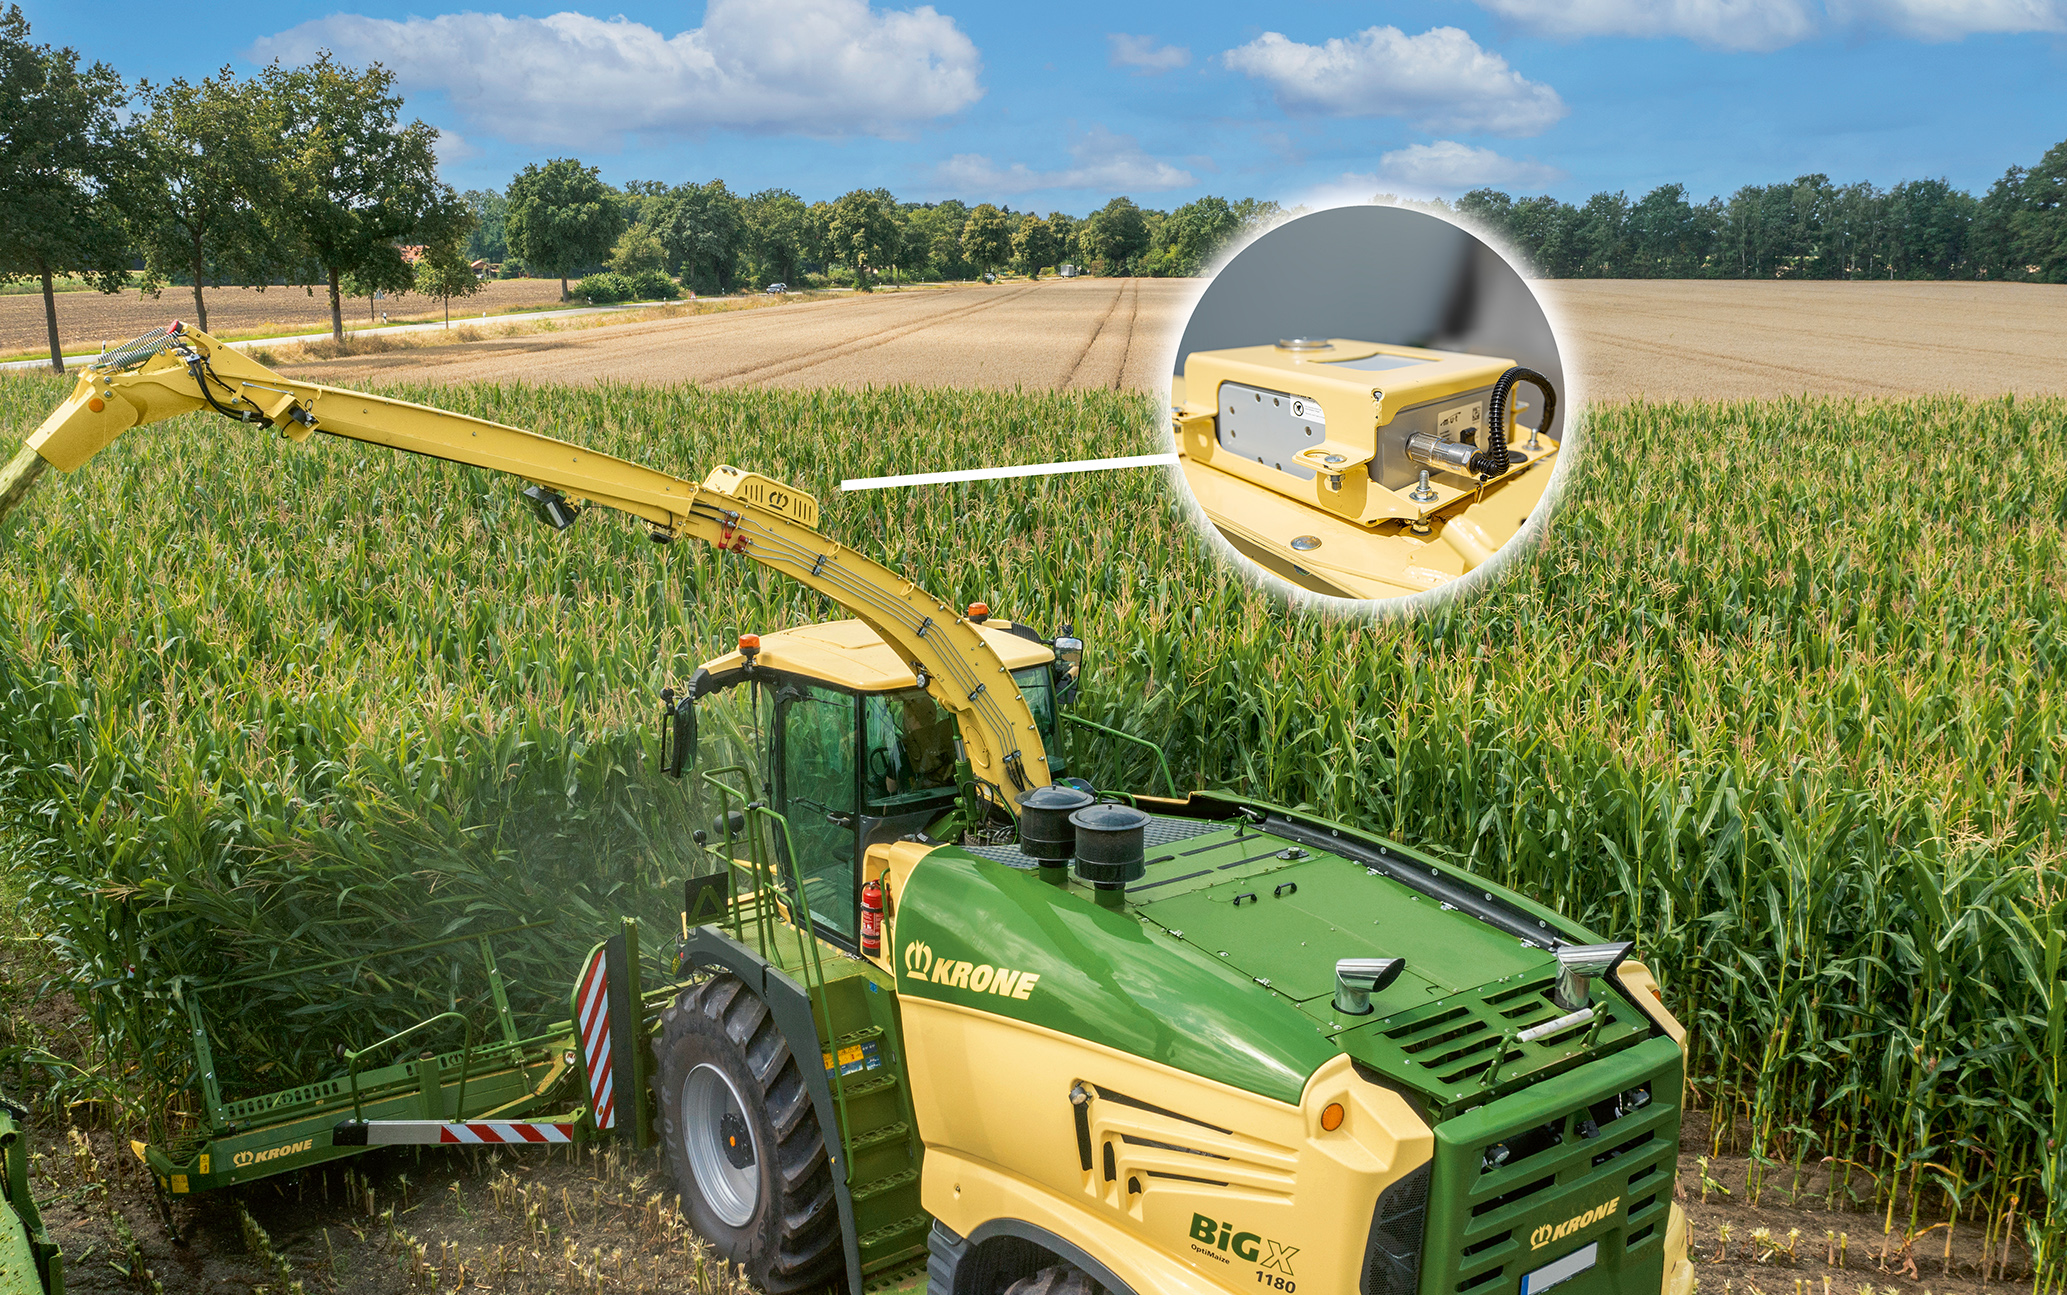
\includegraphics[width=0.7\textwidth]{bilder/Krone NIR Control dual.jpg}
	\caption[Mähhdrescher mit NIR-Sensor]{NIR-Sensor am Mähdrescher \cite{Krone}}
	\label{fig:Mähhdrescher NIR-Sensor}
\end{figure}

Er dient in diesem Fall der Überwachung der Feuchtigkeit des Saatguts,
um dieses vor Schimmel zu schützen.